\section{Badlands National Park}

\subsection{Current Grassland Management Goals and Programs}

\subsubsection{Grassland Management Goals}

\paragraph{Native Mixed Grass Prairie.} The park purpose includes protections of cultural and ecological resources. 
A bulleted list of management priorities begins with the unique landforms and scenery of the Badlands and the preservation of paleontological and geological resources. 
The third point discusses preserving natural processes of the mixed-grass prairie ecosystem.
Badlands National Park (BADL) protects the largest mixed-grass prairie within the national park system (Foundation Statement, 2017).
Stated goals during interviews were broad in their scope. 
They include ``maintain a fully functioning ecosystem'' and ``protect the native mixed-grass prairie''. 
With the lack of a vegetation management plan, specific goals are not communicated in writing.
Invasive species are an issue, but achievable goals have not been set. 
The weed management plan, written in 2003, emphasizes specific treatments, but is out of date and should be rewritten.

\paragraph{Grassland Wildlife.} A definitive focus at BADL is wildlife.
Species reintroductions occurred periodically over the last few decades.
This placed staff and budgets focus on species management. 
Interview responses on site focused heavily on species specific wildlife goals naming specific species when asked about overall natural resources management goals. 
Bison, black-footed ferrets and bighorn sheep are a few of the charismatic species that require consistent management to maintain healthy populations. 
Bison and bighorn sheep in particular are popular with visitors. 
Due to this, other divisions have also focused on these more visible species to the avail of the other resources in the park. 
Goals for wildlife management are numerous, but laser focused in their scope of species vigor.

\subsubsection{Grassland Management Programs}

\paragraph{Exotic Plant Management Team.} Region-wide, the exotic plant management team (EPMT) targets invasive species using mechanical or chemical treatments. 
The team is stationed and managed from BADL.
This means there is significant use of mechanical and chemical means of exotic removal at BADL. 
The species of most concern at this unit is exotic yellow sweet clover. 
Annual bromes continue to be an issue with an Annual Brome Adaptive Management (ABAM) study ongoing in MWR units.
Budgets have reduced the impact that the EPMT can have on landscapes within BADL.

\paragraph{Fire Program.} The fire management plan at BADL was written in 2004. 
This plan split BADL into two management units, the ``Boundary FMU'' and the ``Natural FMU''. 
The ``Boundary FMU'' uses only suppression and prescribed fire whereas the ``Natural FMU'' allows some naturally ignited fires to burn under supervision.
Goals of the 2004 fire management plan include enhancing productivity of the native grasses, decrease the spread of some exotic species and controlling woody species. 
The program discusses restoring fire to 80\% of the vegetated landscape within 15 years of 2004, and restoring a mosaic of grassland seral stages to the landscape.

\paragraph{Wildlife Management Program.} As stated previously, a substantial amount of Park resources are directed towards wildlife management. 
The amount of projects related to wildlife management warrants its status as a program within the Natural Resources division at BADL. 
This program conducts yearly data collection of species within the unit and population roundups to assess species composition. 
Visitor experience at BADL is also centered on the wildlife management program with ``unparalleled views of native wildlife'' present in the park (Foundation Statement, 2017). 
This has allotted more funding towards the wildlife program from higher up sources in the unit and the region. 
The NRCA states that overall wildlife is populations are doing well, with the exception of plague contractions in the black footed ferret populations.

\subsection{Management Plans and Data Available}

\subsubsection{Management Plans}

Several management plans are older and were collected or published before BADL lost a significant amount of staff.
Evidence of this is shown in that three key management plans are not displayed in our table as they are outdated by our year parameters: Fire management plan (2004), general management plan (2006), and Black tailed prairie dog
plan (2007). 
Across the NPS, general management plans are being phased out and replaced by foundation documents (2017), but an updated fire management plan should be of priority as climactic drivers are altering the effects that fire has on landscapes. 
The Natural Resource Condition Assessment (2018) is also extremely relevant.
A complete list of published management plans for BADL can be seen in Table~\ref{tab:BADLManDocs}.

\begin{table}[h]
	\centering
\caption[BADL management documents]
	{Management documents for Badlands National Park published from 2008-2018.} 
\label{tab:BADLManDocs}
\begin{tabular}{lc}
\toprule
Title & Year\tabularnewline
\midrule
Prairie Dog Management Plan & 2008 \tabularnewline
Memorandum of Understanding for Wildland Fire Management & 2008 \tabularnewline
Genetic Based Management Plan for Bison & 2008 \tabularnewline
Climate Change Vulnerability Assessment & 2012 \tabularnewline
Bison Management Plan and EA & 2016 \tabularnewline
Foundation Document & 2017 \tabularnewline
Grasshopper and Mormon Cricket EA  & 2017 \tabularnewline
Natural Resource Condition Assessment & 2018 \tabularnewline
Wilderness Stewardship Plan & 2018 \tabularnewline
South Dakota Bighorn Sheep Management Plan & 2018-2022 \tabularnewline
\bottomrule
\end{tabular}
\end{table}

\subsubsection{Data Available}

Our data audit includes studies from 2008-2018 (Table~\ref{tab:BADLdata}), but a complete list of data beyond our year parameters can be accessed from the NRCA. 
Evident, is the focus of budget, time and staff at BADL. 
Ten of the 18 studies in this table are focused on wildlife and the viability of the protected species within the park.
Vegetation management data is collected by I\&M as the park has no botanist. 
I\&M data is a resource the unit must use to make decisions pertaining to the prairie. 
Community composition data and fire effects data are present in I\&M monitoring documents. 
Data available is scant as told in interviews, the focus with less staff is to just continue managing what they have and not lose anything they have now rather than take on new projects and new data collection.

%\storeareas\normalsetting
\KOMAoption{paper}{landscape}
\areaset{1.5\textwidth}{.6\textheight}
\recalctypearea
\pagestyle{plain}
\setlength\LTcapwidth{1.5\textwidth} 
\setlength\LTleft{0pt}           
\begin{longtable}[l]{@{}p{5cm}p{2cm}p{3cm}p{4cm}p{3cm}p{4cm}p{3cm}@{}}
\caption[BADL data]
{Selected data collected in BADL, 2008-2018.} 
\label{tab:BADLdata} \\
\toprule
Data title & Data type & Spatial extent & Frequency & Duration & Collecting agency & Format located \tabularnewline
\midrule
\endfirsthead 
\caption* {\textbf{Table \ref{tab:BADLdata}}, \emph{continued.}} \\
\toprule
Data title & Data type & Spatial extent & Frequency & Duration & Collecting agency & Format located \tabularnewline
\midrule
\endhead
Mapping of Nutrient- Nitrogen Critical Loads for Selected National Parks in the Intermountain West and Great Lakes Region & Air & park wide & Assessed once via vegetation maps of park units & 2016 & E\&S Environmental Chemistry, Inc./ NPS Air Resources Division & IRMA\tabularnewline
Resource Management Annual Report 2016 & All & park wide & Collections each year & 2016 & NPS & on site at BADL\tabularnewline
Climate Change Vulnerability Assessment & Climate & Park wide & Historical Assessment & Historical-2012 & NPS & IRMA~\tabularnewline
Erosion Rates & Geology & park wide & fall 2010 and 2011 & 2010-2011 & South Dakota School of Mines and Technology & IRMA\tabularnewline
Geologic Maps of BADL & Geology & Park wide & Once & Published 2008 & NPS Geologic Resources Division & IRMA\tabularnewline
Exotic Plant Management Team Achievements & Vegetation & varying acres treated per summer & summer season & have reports from 2003-2011 & NPS EPMT & on site at BADL\tabularnewline
Plant Community Composition & Vegetation & 127 plots across the park & each plot visited for two consecutive years and then rested for eight years on a ten year rotating basis & 2011-current & NGPFire and NGP I\&M & IRMA\tabularnewline
Northern Great Plains Fire Ecology Annual Report & Vegetation & Park wide & annually & 1996-current & NPS Fire Effects Team & IRMA\tabularnewline
Bison weights from National Parks in the Northern Great Plains. & Wildlife & bison herds at three parks & once each fall in each year of collection & 1983-2014 & NPS & online\tabularnewline
Monitoring the birds of Badlands National Park: 2011 report & Wildlife & 25 cells in the north unit of BADL~ & One season & 22 May \textendash 8 July 2011 & Rocky Mountain Bird Observatory & IRMA\tabularnewline
Land bird Monitoring & Wildlife & 161 points across the park & annually & 2012-current & NGP I\&M & IRMA\tabularnewline
Conservation assessment and conservation strategy for swift fox in the United States\textemdash 2011 update & Wildlife & United States & Historical assessment & 1992 \textendash 2011 & South Dakota Game Fish and Parks & Online
search\tabularnewline
Swift Foxes in Southwestern South Dakota: Assessing the Current Status of a Reintroduced Population & Wildlife & Seven-county area of SD & 1000 scent stations established once per year for two years & 2014\textendash 2016 & South Dakota State University  & Online search \tabularnewline
2016 Bighorn Sheep Population Status & Wildlife & opportunistic counts combined with trail camera & 50 hours & 1996-2016 & NPS & on site\tabularnewline
2016 Breeding Bird Survey & Wildlife & three routes & 3 minutes per stop (50 stops) once each year on each route & 2016 & NPS & on site\tabularnewline
Acoustic Surveys of Bats & Wildlife & park wide & 4-7 consecutive nights at each point & 2014-2016 & NPS NGP I\&M & IRMA\tabularnewline
Observations of Bobcats, \emph{Lynx refus}, Hunting Black-tailed prairie dogs, \emph{Cynomys ludovicianus}, in Western South Dakota & Wildlife & Park wide & Winters of 2009-2010 & 2008-2010 & NPS & IRMA\tabularnewline
Grazing Resources for Integrated Conservation of Bison and Native Prairie at Badlands National Park, South Dakota & Wildlife and Vegetation & Park wide & Different aspects of study occurring over three years & Ongoing & USGS & On site\tabularnewline
\bottomrule
\end{longtable}
\clearpage
\normalsetting
\pagestyle{fancy} 

\begin{figure}
\centering
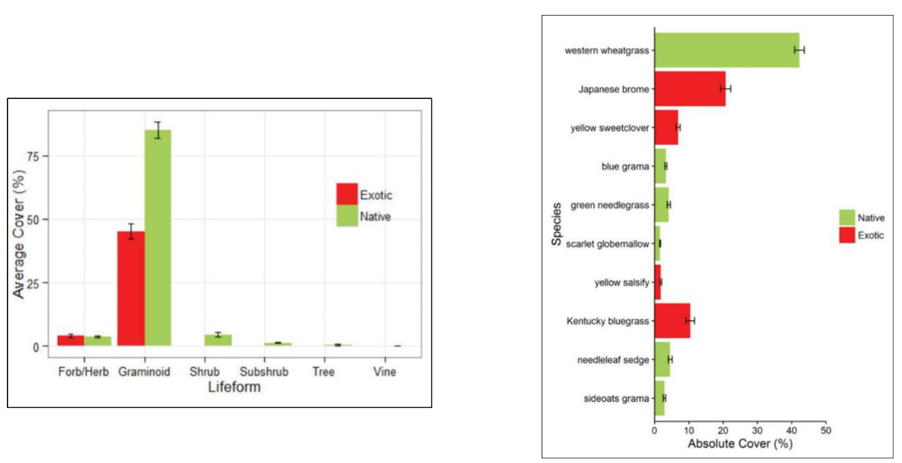
\includegraphics[width=0.75\textwidth]{BADL_veg}
\caption{Vegetation status of BADL prairie 2015 (Ashton and Davis, 2016)}
\label{BADLveg}
\end{figure}


\subsection{Disturbance Regime }

\subsubsection{Grazing }

Livestock grazing was prevalent in the area before BADL establishment.
Livestock grazing also occurred in the park from 1942- 1962.
Bison reintroduction began in 1963, with more animals added in 1983. 
The park currently manages for around 1,000 bison. 
BADL strives for 40\% stocking rate. 
Bighorn sheep, pronghorn and mule deer also contribute to grazing disturbance, but bison are the main conservation herd. 
Bison are currently maintained in one pasture (Fig.~\ref{fig:BADLbison}). 
This constrains their natural movements across the landscape, although a bison expansion project is planned for the coming years (from interviews, this seems to be mostly motivated by enhancing visitor experience pertaining to bison viewing). 
Park reports state that a grazing disturbance has had a positive impact on the landscape. 
Native species richness is higher in pastures containing bison (Ashton and Davis, 2016).

\begin{figure}
	\centering
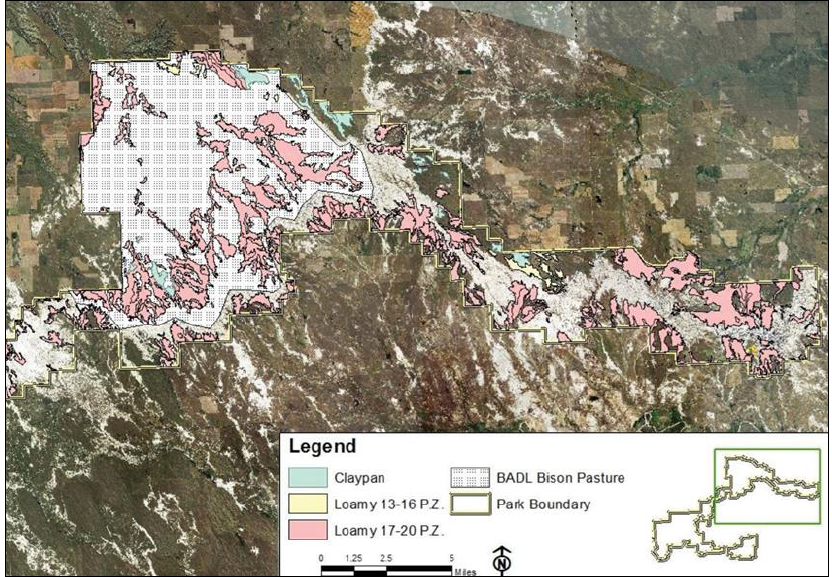
\includegraphics[width=0.75\textwidth]{BADL_Bison_Pasture}
\caption{Bison pasture at BADL and corresponding ecological sites (Ashton and Davis, 2016)} 
\label{fig:BADLbison}
\end{figure}

The eastern edge of the park where grazing and fire are underutilized due to the threat to visitors, the litter layer is in excess inhibiting the vitality of the prairie. (Interview, 2018)

\subsubsection{Fire }

Fire operations for the region are stationed at BADL.
Similar to the EPMT, this means resources are easily available for dispatching to prescribed fires. 
The area has evolved with the use of fire as a disturbance and historical disturbance regimes included fire return
intervals of five years on ``level to gently rolling topography'' and 15-30 years on ``more broken topography'' within the park. 
In the 20\textsuperscript{th} century, suppression was the norm for all fires.
As mentioned earlier, the fire management program changed slightly with the use of a management area where naturally ignited fires are allowed to burn under supervision.
Prescribed fires have created a mosaic of burned patches across the unit from the 1980's until 2012 (Fig.~\ref{fig:BADLfire}), but recently, funding constraints inhibited the use of prescribed fire in BADL (Foundation Statement, 2017). 
Annual brome has increased in patches not recently burned. 
To achieve BADL's grassland management goal of a native mixed-grass prairie with few invasive species, disturbances, such as fire, must be used.

\begin{figure} 
\centering
\includegraphics[width=0.75\textwidth]{BADL_Fire_Mosaic}
\caption{Fire mosaic created by patch burning in BADL (Ashton and Davis,
2016)}
\label{fig:BADLfire}
\end{figure}

BADL knows the importance of a coupled disturbance regime, but implementation has not occurred. 
One report notes that ``fire and grazing alone consistently do not perform adequately to accomplish management objectives,'' and goes on to say that the coupling of the two to create the native disturbance regime is necessary to the maintenance of the prairie, ``grazing regulates fire, fire regulates transitions (to altered plant community composition states)''. 
Spatial and temporal heterogeneity are cited as being important to maintain native processes on the landscape.

\subsection{Data gaps and suggested research}

\subsubsection{Data Gaps}

Data from BADL are focused on wildlife. 
There is a lot of information on wildlife presence or absence as well as vigor with frequent captures and monitoring of wildlife populations. 
Vegetation data for the unit is completely reliant on the I\&M network.
Although this is extremely beneficial data, the monitoring done by the network has no strength in proving cause and effect. 
Studies done in the park either by outside researchers or staff personnel would be beneficial to best understand what varied intensities of disturbance would do to the extremely diverse landscape of BADL.

The recently published NRCA and Foundation Document have cited several data and plan gaps that we would like to echo. 
Most importantly, to establish a disturbance regime, knowledge of the effects of disturbance on your landscape are critical. 
This includes vegetation effects (both native and non-native), erosion rates due to grazing, understanding of your landscape at the soil level with ESD descriptions, and tracking of grazers across a landscape to understand their grazing preferences. 
The inherent heterogeneity of BADL makes this information important so that the imposed heterogeneity through a disturbance regime works positively to enhance ecosystem resilience.

\subsubsection{Suggested Research}

Future research should be focused on how disturbance interacts with the landscape at BADL. 
Fortunately, BADL has two studies underway looking at these interactions. 
The first is studying the effect of grazing on vegetative resources. 
This study will help establish stocking rates, written about in the 2017 Foundation Statement as a gap in data. 
The second is tracking bison across the landscape. 
BADL, WICA and THRO are using GPS collars for bison (as well as other large ungulates) to track their movement in the unit. 
This is used for understanding plant community use by grazers. 
The effect of grazing is being investigated.
Priority is also needed on other disturbances. 
Beneficial studies would be:

\begin{itemize}
\item
  The effect of fire on exotic yellow sweet clover
\item
  The fire return interval for burn units in light of changing climactic
  factors
\item
  The use of fire and the movement of large grazers in response
\item
  Beneficial coupling of the inherent BADL heterogeneity and imposed
  heterogeneity via fire
\item
  Coupling the known erosion rates and ungulate movement to determine
  grazer impact
\end{itemize}

\subsection{Management Recommendations: Prioritize fire in staff and funding}

Current staff and budget priorities at BADL are wildlife related.
Species reintroductions have required staff to allot lots of time to these projects. 
As such, other resources have been managed on minimal budgets and personnel.
This has also prompted the need of partnerships with outside agencies or funding organizations to accomplish tasks within the park which is not always guaranteed money. 
The fire management program has severely suffered from lack of prioritization.
Over the last five years, there has been one prescribed burn in BADL. 
To create a heterogeneous landscape via a disturbance regime, a piece of the landscape needs to be burned each year. 
Bison can also be moved through a landscape by attracting them to recently burned patches. 
This aids in the management of grazers constrained within a fenced pasture so that certain areas are not grazed too heavily. 
This can limit the amount of staff timing to move bison via horseback or helicopter.

To burn each year under a strapped budget, there needs to be forethought of when in the season a burn should occur. 
Vegetation monitoring may suggest that to achieve certain invasive species management goals there needs to be fall prescribed burns. 
This may be unrealistic with staff and budget constraints. 
Spring burning may be required to create a mosaic of different grass stands to best benefit wildlife and other ecosystem processes. 
Spring burning is beneficial for targeting annual bromes when they emerge before native species. 
It also allows the unit to maintain a full crew of firefighters before they have exceeded their hours fighting fires across the United States.
